\chapter{Formulating Language Models as Weighted Sums}
\label{ch:weightedsum}

\todo{Introduce notation: (1) N-Gram length (absolute bars) (2) N-Gram
concatenation (side by side or with star) (3) Empty N-Gram (epsilon).}
This chapter will show how to represent  $\ProbMKN{w_n}{w_1^{n-1}}$ and
$\ProbGLM{w_n}{w_1^{n-1}}$ as weighted sums of terms depending on $w_n$ for a
fixed history $h = w_1^{n-1}$ and an  arbitrary probability event $w = w_n$.
In other words we will express the formulas given in \cref{ch:review} as
equations of the following form:
\begin{equation}
  \label{eq:weightedsum}
  \Prob{w}{h} = \sum_{i = 1}^{N} \SumWeight_i^h \cdot \SumArg_i^h(w_n)
\end{equation}

Being able to accurately represent probabilities in a form like this is highly
beneficial for word prediction.
As we can see in \cref{eq:prefixquery} the computation for next word prediction
is based on calculating multiple probabilities $\Prob{w}{h}$ with a fixed
history $h$ but varying arguments $w$.
As has been specified in \cref{ch:review} probability calculation is based on
complex recursive formulas.
Using our weighted sum representation this computation can be speed up by
a huge factor since computation of the sum weights $\SumWeight^h_i$ can
be performed once beforehand.
For each final probability we then only have to perform the $N$ remaining
lookups $\SumArg^h_i(w)$ that actually depend on $w$.

Another handy benefit is that by this representation we have all terms that
change with $w$ explicitly available, which is a prerequisite for top-$k$
joining and will be explained in \cref{ch:topkjoin}.
Lastly our algorithms for calculating sum weights turn out to be performing
faster
then the direct recursive implementations.
We will measure that effect in \cref{sec:evaluation-probability}.

We will now present the basic idea of how to transform $\Prob{w_n}{w_1^{n-1}}$
into weighted sums, that applies to both Modified Kneser-Ney Smoothing and
the Generalized Language Model:

Note that in all \cref{eq:mkn-high,eq:mkn-low,eq:glm-high,eq:glm-low} the
probability event $w_n$ only appears in the nominator of fractions, specifically
in the argument terms of $\DiscountedCount$ or $\DiscountedCount*$.
Additionally $w_n$ occurs as arguments for $\Count$ and $\ContCountIp$ in the
lowest order \cref{eq:mkn-lowest,eq:glm-lowest}.
Our general idea is thus, to first expand recursive calls to
$\Prob(\DummyArg)$ or $\Prob*(\DummyArg)$, and second to factor
out those terms that do not depend on $w_n$ by the distributive property.

\Cref{sec:weightedsum-mkn} discusses our aprroach for Modified Kneser-Ney
smoothing, while \cref{sec:weightedsum-glm} deals with the Generalized
Language Model.


% ------------------------------------------------------------------------------
\clearpage
\section{Modified Kneser-Ney Smoothing}
\label{sec:weightedsum-mkn}

Modified Kneser-Ney Smoothed probabilities $\ProbMKN{w}{h}$ are calculated as
follows:
\begin{enumerate}
  \item Backing-off: Leave out words at the beginning of the history $h$, until
    $h \Skp$ is seen for the first time (\cref{eq:mkn-backoff}).
  \item Highest order: Take frequency counts $\DiscountedCount(h \: w)$ and
    $\Count(h \Skp)$ (\cref{eq:mkn-high}) and shorten the history by one word.
  \item Lower orders: Take continuation counts $\DiscountedCount*(\WSkp h \: w)$
    and $\ContCountIp(\WSkp h \WSkp)$ (\cref{eq:mkn-low}) and shorten the
    history further until it is empty.
  \item Lowest order: Take continuation counts $\ContCountIp(\WSkp w)$ and
    $\ContCountIp(\WSkp \WSkp)$ (\cref{eq:mkn-lowest}).
\end{enumerate}

\newcommand{\ProbMKNcab}[1]
  {\frac{\DiscountedCount(w_1 w_2 w_3) + \gamma(w_1 w_2) #1}{\Count(w_1 w_2 \Skp)}}
\newcommand{\ProbMKNcb}[1]
  {\frac{\DiscountedCount*(\WSkp w_2 w_3) + \gamma(w_2) #1}{\ContCountIp(\WSkp w_2 \WSkp)}}
\newcommand{\ProbMKNc}
  {\frac{\ContCountIp(\WSkp w_3)}{\ContCountIp(\text{\WSkp \WSkp})}}

As an example we will give the full formula expansion necessary to calculate
$\ProbMKN{w_3}{w_1 w_2}$ for any sequence $w_1 w_2 w_3$, assuming that sequence
was seen:
\begin{subequations}
  \begin{align}
    \ProbMKN {w_3}{w_1 w_2} &= \ProbMKNcab{\ProbMKN*{w_3}{w_2}} \\
    \ProbMKN*{w_3}{w_2}     &= \ProbMKNcb{\ProbMKN*{w_3}} \\
    \ProbMKN*{w_3}          &= \ProbMKNc
  \end{align}
\end{subequations}
Inserting the lower orders results in:
\begin{equation}
  \ProbMKN {w_3}{w_1 w_2} = \ProbMKNcab{\ProbMKNcb{\ProbMKNc}}
\end{equation}
By using the distributive property we obtain:
\begin{align}
  \label{eq:probmknexpansion-final}
  \hspace{-2.5em}\ProbGLM {w_3}{w_1 w_2} = {}
    & & \DiscountedCount (w_1 w_2 w_3)   & \cdot\ \frac{1}{\Count(w_1 w_2 \Skp)} \\
    &+& \DiscountedCount*(\WSkp w_3 w_3) & \cdot\ \frac{\gamma(w_1 w_2)}{\Count(w_1 w_2 \Skp) \ContCountIp(\WSkp w_2 \WSkp)} \nonumber \\
    &+& \ContCountIp(\WSkp w_3)          & \cdot\ \frac{\gamma(w_1 w_2) \: \gamma(w_2)}{\Count(w_1 w_2 \Skp) \ContCountIp(\WSkp w_2 \WSkp) \ContCountIp(\WSkp \WSkp)} \nonumber
\end{align}

In the final equation \cref{eq:probmknexpansion-final} we can clearly see
those terms that do depend on $w$ and those that do not.
Per line the left part of the multiplication dot are the terms $\SumArg^h_i(w)$,
while the terms on the right form the sum weights $\SumWeight^h_i$.

But note that this is only valid if the sequence $w_1 w_2 w_3$ was seen in
the training corpus, that is $\Count(w_1 w_2 w_3) \geq 1$.
If this is not the case, backoff steps have to be performed, and a different
resulting formula is obtained.

All counts except those of the lowest order are discounted using
$\DiscountedCount$ and $\DiscountedCount*$ to interpolate that order with the
following by the weight $\gamma(h)$.
This process of interpolating different orders is visualized in
\cref{fig:history-mkn} for the case of a history of length three.
Building similiar graphs for other history lengths is straightforward.

\begin{figure}[tb]
  \centering
  \documentclass{standalone}
\usepackage[dvipsnames,svgnames,x11names]{xcolor}
\usepackage{tikz}
\usepackage{../thesismath}
\begin{document}
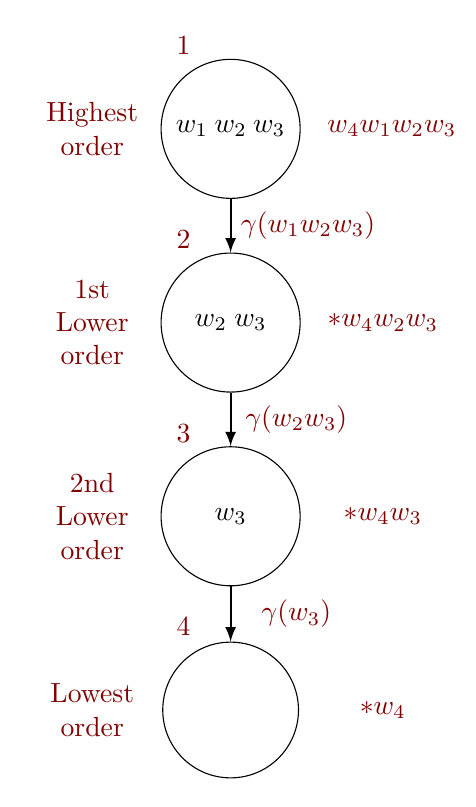
\begin{tikzpicture}
  \tikzset{
    state/.style  = {draw, circle, align = center, text centered, text width = 4.2em},
    invis/.style  = {text width = 4.2em},
    order/.style  = {align = center, text centered, text width = 4em, text = Maroon},
    number/.style = {xshift = -1.7em, text = Maroon},
  }

  \begin{scope}[node distance = 7em]
    \node [state] (highest)                    {$w_1 \: w_2 \: w_3$};
    \node [state] (lower1)  [below of=highest] {$w_2 \: w_3$};
    \node [state] (lower2)  [below of=lower1]  {$w_3$};
    \node [state] (lowest)  [below of=lower2]  {$\EmptyNGram$};
  \end{scope}

  \begin{scope}[node distance = 5.5em]
    \node [order] [right of=highest] {$\ProbMKN {w_4}{w_1 w_2 w_3}$};
    \node [order] [right of=lower1]  {$\ProbMKN*{w_4}{w_2 w_3}$};
    \node [order] [right of=lower2]  {$\ProbMKN*{w_4}{w_3}$};
    \node [order] [right of=lowest]  {$\ProbMKN*{w_4}$};
  \end{scope}

  \begin{scope}[node distance = 5em]
    \node [order] [left of=highest] {Highest order};
    \node [order] [left of=lower1]  {1st Lower order};
    \node [order] [left of=lower2]  {2nd Lower order};
    \node [order] [left of=lowest]  {Lowest order};
  \end{scope}

  \begin{scope}[node distance = 3em]
    \node [number] [above of=highest] {1};
    \node [number] [above of=lower1]  {2};
    \node [number] [above of=lower2]  {3};
    \node [number] [above of=lowest]  {4};
  \end{scope}

  \path[->, >=latex, thick]
    (highest) edge node [right, order] {$\textstyle{\gamma(w_1 w_2 w_3)}$} (lower1)
    (lower1)  edge node [right, order] {$\textstyle{\gamma(w_2 w_3)}$}     (lower2)
    (lower2)  edge node [right, order] {$\textstyle{\gamma(w_3)}$}         (lowest);
\end{tikzpicture}
\end{document}

  \caption{
    Interpolation of different orders during computation of
    $\ProbMKN{w_4}{w_1 w_2 w_3}$.
    Centered are the histories for each probability.
    It is assumed that the history $w_1 w_2 w_3$ was seen during training, so
    that no backing-off is necessary.
    Orders are combined with with interpolation weights $\gamma(\DummyArg)$.
  }
  \label{fig:history-mkn}
\end{figure}

Each order with a history $h$ is interpolated with the following order where
the first word of $h$ is removed.
Thus a total ordering on the histories of the orders can be specified.
In \cref{fig:history-mkn} we have thus assigned each history a number from
$1$~to~$4$.
Let $\DerivedHistory[i]$ denote the history of that graph with number $i$.

The first step in expressing $\ProbMKN{w}{h}$ as a weighted sum is finding the
number $N$ of sum weights.
In the case of Modified Kneser-Ney Smoothing this is exactly the number of
interpolation orders.
Let $\DerivedHistory[s]$ be the first seen history that is the result of
backing off given history $h$ exaclty $s$ many times.
The number $N$ of sum weights is then the number of words of that history plus
one for the empty history.
\begin{equation}
  N = \NGramLength{\DerivedHistory[s]} + 1
\end{equation}
Where $\NGramLength{w_1^n} = n$ is the length of the $n$-gram $w_1^n$.

The next step is to find the actual terms $\SumArg_i^h(w)$ that shall be
weightedly added.
When looking at the equations that define Modified Kneser-Ney we note the fact
that only the count terms in the numerators depend on the probability event $w$.
Exactly these terms compose our sum arguments:
\begin{equation}
  \SumArg_i^h(w) =
    \begin{dcases*}
      \Count(w)                                             & if $N = 1$ \\
      \DiscountedCount(\DerivedHistory[s] w)                & if $N \neq 1 \land i = 1$ \\
      \DiscountedCount*(\WSkp \DerivedHistory[s + i - 1] w) & if $N \neq 1 \land 1 < i < N$ \\
      \ContCountIp(\WSkp w)                                 & if $N \neq 1 \land i = N$
    \end{dcases*}
\end{equation}

Lastly we need to define the actual sum weights $\SumWeight_i^h$.
We note that --- because each order is interpolated with the weight $\gamma$ of
the previous order --- each order is in total weighted by the product of the
$\gamma$s of all previous orders.
Additionally lower order models occur in the numerators of fractions, because of
that they are weighted by all previous denominator counts as well.
Building on this we can define:
\begin{equation}
  \label{eq:mkn-sumweight}
  \SumWeight_i^h = \frac{1}{\Count(\DerivedHistory[s] \Skp)} \prod_{j = 2}^i \frac{\gamma(\DerivedHistory[s+i-2])}{\ContCountIp(\WSkp \DerivedHistory[s+i-1] \WSkp)}
\end{equation}

Specifying an algorithm to compute interpolation weights $\SumWeight_i^h$ that
minimizes frequency count lookup (using the iterative definition of
$\SumWeight_i^h$) is straightforward and given in \cref{alg:weightedsum-mkn}.
In \cref{ln:alg-mkn-lowerorders} the lower order sum weights are assigned.
It takes advantage of the fact that \cref{eq:mkn-sumweight} can easily be
written in a recursive manner.
This is done to avoid repeated count lookups and multiplications.

\begin{algorithm}
  \caption{Computing Modified Kneser-Ney sum weights}
  \label{alg:weightedsum-mkn}
  \begin{algorithmic}[1]
    \Require $h$
      \Comment{history for which to determinate sum weights}
    \Ensure $\SumWeight_1^h, \: \ldots, \: \SumWeight_N^h$
      \Comment{list of sum weights}

    \LineComment{find first seen history}
    \State $s \gets 1$
    \While{$\Count(\DerivedHistory[s] \Skp) = 0$}
      \Comment{while history is unseen}
      \State $s \gets s + 1$
    \EndWhile

    \vspace{0.7em}
    \LineComment{compute sum weights}
    \State $N \gets \NGramLength{\DerivedHistory[s]} + 1$
      \Comment{number of sum weights}
    \vspace{0.1em}
    \State $\SumWeight_1^h \gets \dfrac{1}{\Count(\DerivedHistory[s] \Skp)}$
      \Comment{set weight of highest order}
    \For{$i$ \textbf{from} $2$ \textbf{to} $N$}
      \State $\SumWeight_i^h \gets \SumWeight_{i-1}^h \dfrac{\gamma(\DerivedHistory[s + i - 2])}{\ContCountIp(\WSkp \DerivedHistory[s + i - 1] \WSkp)}$
        \Comment{weight of lower orders}
        \label{ln:alg-mkn-lowerorders}
    \EndFor
  \end{algorithmic}
\end{algorithm}


% ------------------------------------------------------------------------------
\section{Generalized Language Model}
\label{sec:weightedsum-glm}

The difference between a Modified Kneser-Ney language model and a
Generalized Language Model is the way in which orders are interpolated.
Instead of just one probability --- that of shortening the history by one ---
being factored in, in the Generalized Language Model the average of multiple
probabilities of the next lower order is factored into the higher order
probability.

This section will not consider the general case were one probability
$\ProbGLM{w}{h}$ incorporates exactly $\NumSkpOp{h}$ probabilities
$\ProbGLM*{w}{\SkpOp[j]{h}}$ of the next lower order.
Instead only the special case described by \textcite{Pickhardt2014}, that is
actually used in practice, is examined.
That is the number of lower order probabilities incorporated $\NumSkpOp{h}$
is set to the number of non-skip words in $h$, and $\SkpOp[j]{h}$ is defined as
replacing the $j$th non-skip word in $h$ with a skip $\Skp$.

% - - - - - - - - - - - - - - - - - - - - - - - - - - - - - - - - - - - - - - -
\subsection{Binomial Diamond}

\todo[inline]{Do we mention \emph{Hasse diagrams} in this subsection?}
\Rene[inline]{Let us discuss ``Hasse'' vs ``diamond''. Only use one term or the
other.}

The directed graph of \cref{fig:history-glm} visualizes the lower order
probabilities that factor into those of higher orders, using that definition of
$\SkpOp[j]{h}$.
The nodes represent the histories $h$ of a probability $\ProbGLM{w_4}{h}$.
The directed edges represent an immediate dependency, for example the
probabilities that occur in the definition of
$\ProbGLM*{w_4}{w_1 w_2 \Skp}$ are $\ProbGLM*{w_4}{w_1 \Skp \Skp}$ and
$\ProbGLM*{w_4}{\Skp w_2 \Skp}$.

\begin{figure}
  \centering
  \documentclass{standalone}
\usepackage[dvipsnames,svgnames,x11names]{xcolor}
\usepackage{tikz}
\usepackage{../thesismath}
\begin{document}
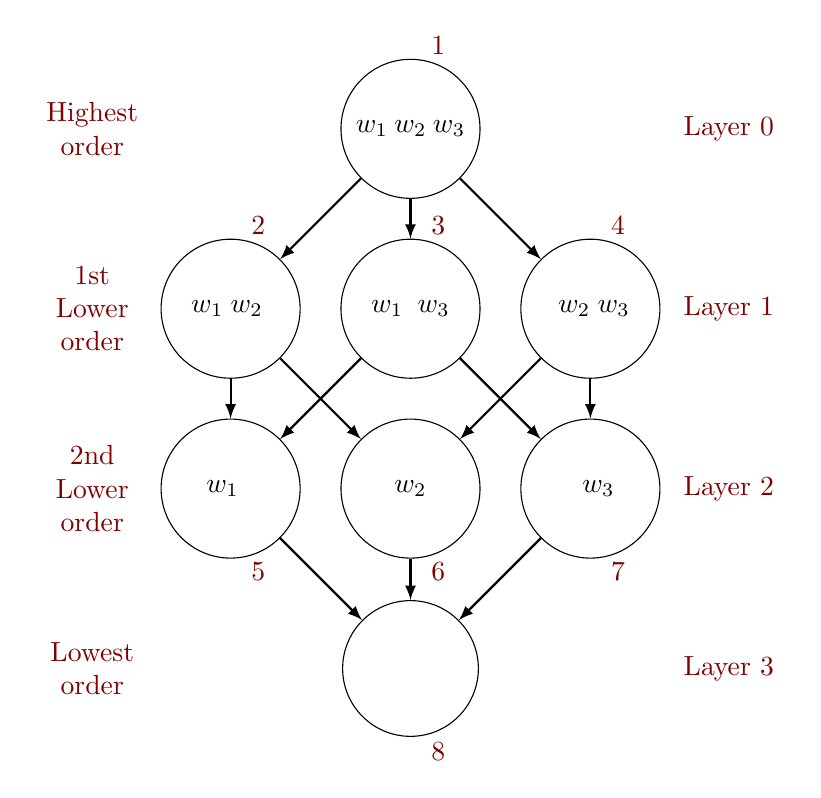
\begin{tikzpicture}
  \tikzset{
    state/.style  = {draw, circle, align = center, text centered, text width = 4.2em},
    invis/.style  = {text width = 4.2em},
    order/.style  = {align = center, text centered, text width = 4em, text = Maroon},
    number/.style = {xshift = 1em, text = Maroon},
  }

  \begin{scope}[node distance = 6.5em]
    \node [state] (000)                  {$w_1 \: w_2 \: w_3$};
    \node [invis] (000l) [left  of=000]  {};
    \node [invis] (000r) [right of=000]  {};

    \node [state] (001)  [below of=000l] {$w_1 \: w_2 \: \Skp$};
    \node [state] (010)  [below of=000]  {$w_1 \: \Skp \: w_3$};
    \node [state] (100)  [below of=000r] {$\Skp \: w_2 \: w_3$};

    \node [state] (011)  [below of=001] {$w_1 \: \Skp \: \Skp$};
    \node [state] (101)  [below of=010] {$\Skp \: w_2 \: \Skp$};
    \node [state] (110)  [below of=100] {$\Skp \: \Skp \: w_3$};

    \node [state] (111)  [below of=101] {$\Skp \: \Skp \: \Skp$};
    \node [invis] (111l) [below of=011] {};
    \node [invis] (111r) [below of=110] {};
  \end{scope}

  \begin{scope}[node distance = 5em]
    \node [order] [left of=000l]  {Highest order};
    \node [order] [left of=001]   {1st Lower order};
    \node [order] [left of=011]   {2nd Lower order};
    \node [order] [left of=111l]  {Lowest order};

    \node [order] [right of=000r] {Layer 0};
    \node [order] [right of=100]  {Layer 1};
    \node [order] [right of=110]  {Layer 2};
    \node [order] [right of=111r] {Layer 3};
  \end{scope}

  \begin{scope}[node distance = 3em]
    \node [number] [above of=000] {1};
    \node [number] [above of=001] {2};
    \node [number] [above of=010] {3};
    \node [number] [above of=100] {4};
    \node [number] [below of=011] {5};
    \node [number] [below of=101] {6};
    \node [number] [below of=110] {7};
    \node [number] [below of=111] {8};
  \end{scope}

  \path[->, >=latex, thick]
    (000) edge (001)
    (000) edge (010)
    (000) edge (100)

    (001) edge (011)
    (001) edge (101)
    (010) edge (011)
    (010) edge (110)
    (100) edge (101)
    (100) edge (110)

    (011) edge (111)
    (101) edge (111)
    (110) edge (111);
\end{tikzpicture}
\end{document}

  \caption{
    Binomial diamond of order 3 for history $h = w_1 \: w_2 \: w_3$.
  }
  \label{fig:history-glm}
\end{figure}

We call a graph that represents the inter-dependencies of probabilities during
the calculation of $\ProbGLM{w}{h}$ the \emph{binomial diamond} of order
$n = \NGramLength{h}$, because of its diamond-like shape, and a number of
properties:

\begin{enumerate}
  \item \label{itm:num-layers} If the graph is partitioned into layers, where
    layer $k$ contains the histories that have exactly $k$ skip words, the graph
    has $n + 1$ layers.
  \item \label{itm:num-childs} Layer $k$ contains exactly $\binom{n}{k}$ nodes.
  \item \label{itm:num-edges}  Nodes in layer $k$ have exactly $n - k$ outgoing
    and $k$ incoming edges.
  \item \label{itm:num-nodes}  There are $2^n$ nodes in the graph.
\end{enumerate}

\Cref{itm:num-layers} is due to the fact that layer $k$ includes exactly those
histories that are part of the $k$th highest order of probability.

To explain \cref{itm:num-childs}, it is helpful to imagine replacing words in
a history as laying a mask of either a skip or a non-skip on top of each word.
\todo{Add small figure to visualize this idea?}
\Rene[noline]{Unnecessary, but if you have time.}
Then the number of nodes in each layer can be understood as permuting the
skip and non-skip masks on top of the history.
It is a well known fact that there are exactly $\binom{n}{k}$ permutations of
$k$ tokens of type A (skips) and $l$ tokens of type B (non-skips) when
$n = k + l$.

\Cref{itm:num-edges} directly follows from the fact, that each non-skip word
in a history can be replaced by a skip, and that each skip is the result
of those replacements.

Lastly, we can explain \cref{itm:num-nodes} because every history is just the
result of laying a mask that is a combination of skips or non-skips on top of
the original history.
All possible masks are then all permutations of two elements (skips or
non-skips) with repetition of length $n$, which there are $2^n$ arrangements of.
We can also infer this from \cref{itm:num-childs} via the binomial theorem
$(x+ y)^n = \sum_{k=0}^n \binom{n}{k} x^{n-k} y^k$, if we set ${x = y = 1}$,
we obtain $\sum_{k=0}^n \binom{n}{k} = 2^n$.

Following the model of the binomial diamond will be a major aid in understanding
the weighted sum representation of the Generalized Language Model.


% - - - - - - - - - - - - - - - - - - - - - - - - - - - - - - - - - - - - - - -
\subsection{Number of sum weights}

\Rene[noline]{Such announcements are hard to read, either discuss when necessary
or here completely, don't split over multiple pages.}
In the previous subsection, it was reasoned that, in the Generalized Language
Model, for a history of length $n$ there are exactly $2^n$ possible derivative
histories.
Following this, one might make the assumption, that to evaluate $\ProbGLM{w}{h}$
it is necessary to evaluate at most $2^n - 1$  different probabilities
$\ProbGLM*{w}{\partial^* h}$ where $\partial^* h$ is any of the $2^n - 1$
derived histories of $h$ excluding $h$ itself.
This assumption however is wrong as it can be necessary that one history $h^*$
is both part of a highest order probability $\ProbGLM{w}{h^*}$ and a lower order
probability $\ProbGLM*{w}{h^*}$ in the presence of unseen histories, as will
shown in the next paragraph.

\begin{subequations}
  Let us for example calculate the probability $\ProbGLM{c}{a \: b}$ on
  hypothetical training data. Were the history $a b$ not to occur in that training
  corpus, we would have to substitute the average of back-off probabilities
  following \cref{eq:glm-backoff}:
  \begin{equation}
    \ProbGLM{c}{a \: b} = \frac{1}{2} \left( \ProbGLM{c}{\Skp b} + \ProbGLM{c}{a \Skp}\right)
  \end{equation}
  Note that these back-off probabilities for histories $\Skp b$ and $a \Skp$
  are still of the highest order $\ProbGLM$.
  We now further assume history $\Skp b$ to also not occur in training, so that
  further back-off is necessary.
  History $a \Skp$ however is treated as seen:
  \begin{align}
    \label{eq:glm-example-unseen}
    \ProbGLM{c}{\Skp b} &= \ProbGLM{c}{\Skp \Skp} \\
    \label{eq:glm-example-seen}
    \ProbGLM{c}{a \Skp} &= \frac{\Count(a \Skp \: c) + \gamma(a \Skp) \ProbGLM*{c}{\Skp \Skp}}
                                 {\Count(a \Skp \Skp)}
  \end{align}
  We can see, that both $\ProbGLM{c}{\Skp \Skp}$ (\cref{eq:glm-example-unseen}) and
  $\ProbGLM*{c}{\Skp \Skp}$ (\cref{eq:glm-example-seen}) factor into probability
  $\ProbGLM{c}{a b}$.
  They would be evaluated as:
  \begin{align}
    \ProbGLM {c}{\Skp \Skp} &= \frac{\Count(\Skp \Skp c)}{\Count(\Skp \Skp \Skp)} \\
    \ProbGLM*{c}{\Skp \Skp} &= \frac{\ContCountIp(\WSkp \Skp \Skp c)}{\ContCountIp(\WSkp \Skp \Skp \WSkp)}
  \end{align}
\end{subequations}

Because of this, it is possible that one history $h^*$ might both occur as
highest order probability $\ProbGLM{w}{h^*}$ and lower order probability
$\ProbGLM*{w}{h^*}$.
It is non-trivial to decide exactly how many derived histories occur both as
highest and lower order probabilities, and to fit algorithms to this finding.
Consequently we only employ an upper bound of sum weights $N$ and set all
unnecessary sum weights to zero.
An upper bound for the number of sum weights is the number of derived histories
times two, as histories can occur both in highest and lower order probabilities:
\begin{equation}
  N = 2 \cdot 2^\NGramLength{h}
\end{equation}


% - - - - - - - - - - - - - - - - - - - - - - - - - - - - - - - - - - - - - - -
\subsection{Sum factors}

\begin{subequations}
  \begin{align}
    \SumArg_{2 i - 1}^h(w) &=
      \begin{dcases*}
        \DiscountedCount(\DerivedHistory[i] w)        & if $\NumSkpOp{\DerivedHistory[i]} > 0$ \\
        \Count(\DerivedHistory[i] w)                  & if $\NumSkpOp{\DerivedHistory[i]} = 0$
      \end{dcases*} \\
    \SumArg_{2 i}^h(w) &=
      \begin{dcases*}
        \DiscountedCount*(\WSkp \DerivedHistory[i] w) & if $\NumSkpOp{\DerivedHistory[i]} > 0$ \\
        \ContCountIp(\WSkp \DerivedHistory[i] w)      & if $\NumSkpOp{\DerivedHistory[i]} = 0$
      \end{dcases*}
  \end{align}
\end{subequations}
\Rene{Why no discount in case $\NumSkpOp{\DerivedHistory[i]} = 0$? This isn't
unigram case or is it?}
\todo[inline]{Or alternatively?}
\begin{equation}
  \SumArg_{2 i + j}^h(w) =
    \begin{dcases*}
      \Count(\DerivedHistory[i] w)                  & if $j = 0 \land \NumSkpOp{\DerivedHistory[i]} = 0$ \\
      \ContCountIp(\WSkp \DerivedHistory[i] w)      & if $j = 1 \land \NumSkpOp{\DerivedHistory[i]} = 0$ \\
      \DiscountedCount(\DerivedHistory[i] w)        & if $j = 0 \land \NumSkpOp{\DerivedHistory[i]} > 0$ \\
      \DiscountedCount*(\WSkp \DerivedHistory[i] w) & if $j = 1 \land \NumSkpOp{\DerivedHistory[i]} > 0$
    \end{dcases*}
\end{equation}
\todo[inline]{Or alternatively?}
\begin{equation}
  \SumArg_{2 i + j}^h(w) =
    \begin{dcases*}
      \Count(\DerivedHistory[i] w)                  & if $j = 0 \land N - i \leq 1$ \\
      \ContCountIp(\WSkp \DerivedHistory[i] w)      & if $j = 1 \land N - i \leq 1$ \\
      \DiscountedCount(\DerivedHistory[i] w)        & if $j = 0 \land N - i > 1$ \\
      \DiscountedCount*(\WSkp \DerivedHistory[i] w) & if $j = 1 \land N - i > 1$
    \end{dcases*}
\end{equation}

\begin{draft}
Coefficient $\mu = \frac{(order - level)!}{order!}$.
\end{draft}

\begin{draft}
$\SumWeight_{2 i}^h$ is $\frac{\mu}{\Count(\DerivedHistory[i]) \Skp)}$ times number
of unseen paths to node.

$\SumWeight_{2 i + 1}^h$ is
$\frac{\mu}{\ContCountIp(\WSkp \DerivedHistory[i] \WSkp)}$ times the sum of paths to
node with each node on path weighted.
\begin{enumerate}
  \item Weight unseen nodes as zero if they are direct parents of targets and if
    target is seen.
  \item Else weight unseen nodes as one.
  \item Weight first seen node as $\frac{\gamma(\DerivedHistory[i](h^*))}{\Count(\DerivedHistory[i](h^*) \Skp)}$.
  \item Weight following nodes as $\frac{\gamma(\DerivedHistory[i](h^*))}{\ContCountIp(\WSkp \DerivedHistory[i](h^*) \WSkp)}$.
\end{enumerate}
\end{draft}

\Lukas[inline]{I have no idea for a good notation for this concept of a path in binomial
diamond.}


% - - - - - - - - - - - - - - - - - - - - - - - - - - - - - - - - - - - - - - -
\subsection{Algorithm}

\begin{draft}
Counts usually stored in hash maps, so we get them to avoid look up.

Use fact that we can apply distributive property on common roots in paths for
one node.
\end{draft}

\begin{algorithmic}[1]
  \State node.\Call{count}{$ $} $= \Count(h_\text{node} \Skp)$
  \State node.\Call{contCount}{$ $} $= \ContCountIp(\WSkp h_\text{node} \WSkp)$
  \State node.\Call{gamma}{$ $} $= \gamma(h_\text{node})$
\end{algorithmic}

%\begin{algorithm}
%  \begin{algorithmic}[1]
%    \Function{calcCoefficient}{$level$, $order$}
%      \Rene[inline]{This is cached, right?}
%      \State $\mu = 1$
%      \For{$i \gets 1 \mathinner{\ldotp \ldotp} level$}
%        \State $\mu \gets \frac{\mu}{order - i + 1}$
%      \EndFor
%      \State \textbf{return} $\mu$
%    \EndFunction
%  \end{algorithmic}
%\end{algorithm}

\begin{algorithm}
  \caption{Computing Generalized Language Model sum weights}
  \label{alg:weightedsum-glm}
  \begin{algorithmic}[1]
    \Require $h$
      \Comment{history for which to determinate sum weights}
    \Ensure $\SumWeight_1^h, \: \ldots, \: \SumWeight_N^h$
      \Comment{list of sum weights}

    \State $n \gets \NGramLength{h}$
      \Comment{$n$-gram length of history $h$}
    \State $N \gets 2 \cdot 2^n$
      \Comment{number of sum factors}
    \For{\textbf{each} node \textbf{in} graph}
      \LineComment{precomputation}
      \State node.count $\gets \Count(h_\text{node.index} \Skp)$
      \State node.contCount $\gets \ContCountIp(\WSkp h_\text{node.index} \WSkp)$
      \State node.gamma $\gets \gamma(h_\text{node.index})$
      \State $\mu \gets \frac{(n - \text{node.layer})!}{n!}$

      \vspace{1.0em}
      \LineComment{weight for highest order}
      \If{node.count $= 0$}
        \State $\SumWeight_{2 \cdot\, \text{node.index} - 1}^h \gets 0$
      \ElsIf{node $=$ root}
        \State $\SumWeight_{2 \cdot\, \text{node.index} - 1}^h \gets \dfrac{\mu}{\text{node.count}}$
      \Else
        \State $\SumWeight_{2 \cdot\, \text{node.index} - 1}^h \gets \dfrac{\mu \cdot \text{\Call{absoluteWeight}{root, node}}}{\text{node.count}}$
      \EndIf

      \vspace{0.7em}
      \LineComment{weight for lower orders}
      \If{node.contCount $= 0$}
        \State $\SumWeight_{2 \cdot\, \text{node.index}}^h \gets 0$
      \Else
        \State $\SumWeight_{2 \cdot\, \text{node.index}}^h \gets \dfrac{\mu \cdot \text{\Call{continuationWeight}{root, node, \textbf{true}}}}{\text{node.contCount}}$
      \EndIf
    \EndFor
    \algstore{glmbreak}
  \end{algorithmic}
\end{algorithm}

\begin{algorithm}
  \caption{Helper functions for GLM sum weight computation}
  \label{alg:weightedsum-glm-helper}
  \begin{algorithmic}[1]
    \algrestore{glmbreak}
    \Function{absoluteWeight}{ancestor, node}
      \If{ancestor.count $\neq 0$}
        \Comment{if ancestor is seen}
        \State \textbf{return} $0$
          \Comment{this path does not contribute to highest order}
      \EndIf

      \vspace{0.7em}
      \If{ancestor.\Call{isDirectParentOf}{node}}
        \State \textbf{return} $1$
      \EndIf

      \vspace{0.7em}
      \State sum $\gets 0$
      \For{\textbf{each} child \textbf{in} ancestor.\Call{childs}{$ $}}
        \If{child.\Call{isAncestorOf}{node}}
          \State sum $\gets$ sum $+ {}$ \Call{absoluteWeight}{child, node}
        \EndIf
      \EndFor
      \State \textbf{return} sum
    \EndFunction

    % --------------------------------------------------------------------------
    \vspace{0.7em}
    \Statex\hrule

    \Function{continuationWeight}{ancestor, node, firstSeen}
      \LineComment{calculate mult}
      \If{firstSeen \textbf{and} ancestor.count $\neq 0$}
        \State mult $\gets \frac{\text{ancestor.gamma}}{\text{ancestor.count}}$
        \State firstSeen $\gets$ \textbf{false}
      \ElsIf{ancestor.contCount $\neq 0$}
        \State mult $\gets \frac{\text{ancestor.gamma}}{\text{ancestor.contCount}}$
      \Else
        \State mult $\gets 1$
      \EndIf

      \vspace{0.7em}
      \If{ancestor.\Call{isDirectParentOf}{node}}
        \If{firstSeen}
          \State \textbf{return} $0$
            \Comment{node occurs as highest order for this path}
        \EndIf{}
        \State \textbf{return} mult
      \EndIf

      \vspace{0.7em}
      \State sum $\gets 0$
      \For{\textbf{each} child \textbf{in} ancestor.\Call{childs}{$ $}}
        \If{child.\Call{isAncestorOf}{node}}
          \State sum $\gets$\\
            \hfill sum $+$ \Call{continuationWeight}{child, node, firstSeen}
        \EndIf{}
      \EndFor
      \State \textbf{return} $mult \cdot sum$
    \EndFunction
  \end{algorithmic}
\end{algorithm}

\todo[inline]{Can we improve algorithm if we just walk each path once?}


% - - - - - - - - - - - - - - - - - - - - - - - - - - - - - - - - - - - - - - -
\subsection{Computational Complexity}

\todo[inline]{Find complexity of naive approach.}

\todo[inline]{Find complexity of my algorithm. Need to find complexity of
finding paths for this.}

\Rene[inline]{Finding paths is breath or depth first search. I think you text
fails to differentiate between training and query time. Your whole approach is
to optimize query time, although this is implicit in argmax.}


% - - - - - - - - - - - - - - - - - - - - - - - - - - - - - - - - - - - - - - -
\subsection{Bitmagic}

\todo[inline]{Better subsection name.}
